\documentclass[jou]{apa6}

\usepackage[american]{babel}

\usepackage{csquotes}
\usepackage[style=apa,sortcites=true,sorting=nyt,backend=biber]{biblatex}
\DeclareLanguageMapping{american}{american-apa}
\addbibresource{bibliography.bib}


%%%%%%%%%%%%%%%%%%%%%%%%%%%%%%%%%%%%%%%%
%% Discrete Structures
%% The start of RBS stuff
%%%%%%%%%%%%%%%%%%%%%%%%%%%%%%%%%%%%%%%%

% Working internal and external links in PDF
\usepackage{hyperref}
% Extra math symbols in LaTeX
\usepackage{amsmath}
\usepackage{gensymb}
\usepackage{amssymb}
% Enumerations with (a), (b), etc.
\usepackage{enumerate}

\let\OLDitemize\itemize
\renewcommand\itemize{\OLDitemize\addtolength{\itemsep}{-6pt}}

\usepackage{etoolbox}
\makeatletter
\preto{\@verbatim}{\topsep=3pt \partopsep=3pt }
\makeatother

% These sizes redefine APA for A4 paper size
\oddsidemargin 0.0in
\evensidemargin 0.0in
\textwidth 6.27in
\headheight 1.0in
\topmargin -24pt
\headheight 12pt
\headsep 12pt
\textheight 9.19in

\usepackage{xcolor}


\title{Quiz for Week02}
\author{Discrete Structures, Fall 2020}
\affiliation{RBS}

\leftheader{Discrete Structures (W2): Quiz}

\abstract{%
}

%\keywords{}

\begin{document}

\twocolumn

\section{Quiz 3: First Order Logic}




\vspace{6pt}
{\bf Question 1.} We have the following
truth table. 
Find the correct DNF (Disjunctive Normal Form) expressing $E(X,Y,Z)$.\\
{\em Note.} Multiple answers may be true, since
there may more than one way to write DNFs for the same Boolean 
function.


\begin{tabular}{@{}ll@{}} 
\begin{minipage}{0.33\columnwidth}
\noindent
\begin{tabular}{ c | c | c | c }
$X$ & $Y$ & $Z$ & $E$ \\ \hline
{\tt T} & {\tt T} & {\tt T} & {\tt F} \\ \hline
{\tt T} & {\tt T} & {\tt F} & {\tt F} \\ \hline
{\tt T} & {\tt F} & {\tt T} & {\tt T} \\ \hline
{\tt T} & {\tt F} & {\tt F} & {\tt F} \\ \hline
{\tt F} & {\tt T} & {\tt T} & {\tt T} \\ \hline
{\tt F} & {\tt T} & {\tt F} & {\tt F} \\ \hline
{\tt F} & {\tt F} & {\tt T} & {\tt T} \\ \hline
{\tt F} & {\tt F} & {\tt F} & {\tt F} \\ \hline
\end{tabular}
\end{minipage} &
\begin{minipage}{0.65\columnwidth}

\begin{enumerate}[(A)]
\item $(X \wedge \neg Y \wedge Z) \;\vee\;$\\
$\;\vee\; (\neg X \wedge Y \wedge Z)$.
\item $(\textcolor{red}{\neg X} \wedge Y \wedge Z) \vee (\neg Y \wedge Z)$.
\item $(\neg X \wedge Z) \vee (X \wedge \neg Y \wedge Z)$.
\item $(\neg X \wedge \neg Y \wedge Z) \vee (\neg X \wedge Y)$.
\end{enumerate}

\end{minipage}
\end{tabular}


\vspace{6pt}
{\bf Question 2.} Identify, which is the correct CNF 
(Conjunctive Normal Form) that computes the same thing as 
Peirce's arrow: $a \downarrow b = \neg (a \vee b)$.\\
{\em Note.} Multiple answers may be true, since
there may more than one way to write CNFs for the same Boolean 
function.

\noindent
{\normalsize \bf (A)} %% Fine
$(\neg a \vee \neg b) \wedge (\neg a \vee b) \wedge (a \vee \neg b)$.\\[3pt]
{\normalsize \bf (B)}
$(a \vee b) \wedge (\neg a \vee b) \wedge (a \vee \neg b)$.\\[3pt]
{\normalsize \bf (C)}
$\neg a \vee \neg b$.\\[3pt]
{\normalsize \bf (D)} %% Fine
$\neg a \wedge (a \vee \neg b)$.



\vspace{6pt}
{\bf Question 3.} We have predicates $A(p,i,r)$ (a Python program 
$p \in \mathcal{P}$ receives input $i \in \mathbb{Z}^{+}$ and answers
with the result $r \in \mathbb{Z}^{+}$); $H(p,i)$ (program $p$ halts on input $i$), 
and $C(i,r)$ (the correct/expected output for input $i$ is $r$). 
Identify the predicate expression that expresses the following English sentence:

{\em ``For all inputs that are sufficiently large, the given program $p$ 
halts and produces outputs that are correct; for some (finitely many) inputs $p$ 
may loop forever, but it is never incorrect.''}




\noindent
{\normalsize \bf (A)}
$\forall p \in \mathcal{P}\; \forall i \in \mathbb{Z}^{+}\; \forall r \in \mathbb{Z}^{+},$\\
$((i > M \,\wedge\, H(p,i)) \vee (A(p,i,r) \wedge C(i,r)))$.\\[3pt]
{\normalsize \bf (B)}
$\exists M \in \mathbb{Z}^{+}\; \forall i \in \mathbb{Z}^{+}\;
\exists r \in \mathbb{Z}^{+},$\\
$((i < M \,\wedge\, \neg H(p,i)) \vee (A(p,i,r) \wedge C(i,r)))$.\\[3pt]
{\normalsize \bf (C)}
$\forall p \in \mathcal{P}\; \exists M \in \mathbb{Z}^{+}\; \forall i \in \mathbb{Z}^{+}\;
\forall r \in \mathbb{Z}^{+},$\\
$((i > M \,\wedge\, H(p,i)) \vee (A(p,i,r) \wedge C(i,r)))$.\\[3pt]
{\normalsize \bf (D)}
$\forall p \in \mathcal{P}\; \forall i \in \mathbb{Z}^{+}\;
\forall r \in \mathbb{Z}^{+},$\\
$((i > M \,\wedge\, H(p,i)) \vee (A(p,i,r) \wedge C(i,r)))$.


\vspace{6pt}
{\bf Question 4.} For the quantifiers 
($A(p,i,r)$, $H(p,i)$, $C(i,r)$) defined in the previous question, 
the following expression is given:
$$\forall p \in \mathcal{P}\;
\exists i \in \mathbb{Z}^{+}\; \exists j \in \mathbb{Z}^{+},$$
$$(j > i \,\wedge\, (H(p,i) \rightarrow H(p,j)).$$
Which sentence is expressed by this?

\noindent
{\bf (A)} Each Python program halts for at least 2 inputs.\\
{\bf (B)} Each Python program halts for infinitely many inputs. \\
{\bf (C)} There is no Python program that halts on exactly 1 input. \\
{\bf (D)} For each Pyton program there is the largest input for which it halts.\\
{\color{red} {\bf (E)} The statement is always true (regardless of halting behavior of Python programs).}

\vspace{6pt}
{\bf Question 5.} 
There is a set of 2 students $S = \{ s_1, s_2 \}$ and 
a set of 5 chairs $C = \{ c_1, c_2, c_3, c_4, c_5 \}$. 
Find, how many such functions $f\,:\,S \rightarrow C$ exist (a function 
by definition is a mapping that assigns a chair for each student;
it is NOT always true that different students get different chairs
or that all chairs are occupied). Please find the total number of 
such functions, also the number of injective, surjective
and bijective functions among them.\\
{\em Note.} Your answer should be a comma-separated list of 
4 numbers (and 3 commas).



\vspace{6pt}
{\bf Question 6.} 
Predicate $S(x,y,z)$ is true iff $x \cdot y=z$.
Given the following equation:\\[3pt]
$\forall u \in \mathbb{Z}^{+}\;\forall v \in \mathbb{Z}^{+}\;
\textcolor{red}{\forall d \in \mathbb{Z}^{+}}\;
\forall p \in \mathbb{Z}^{+}\;\forall q \in \mathbb{Z}^{+}\;
\exists k \in \mathbb{Z}^{+},$\\
$S(x,u,y) \wedge S(x,v,z) \wedge
S(d,p,y) \wedge S(d,q,z) \rightarrow S(d,k,x).$


Which statement is expressed by this expression?\\
{\bf (A)} $d$ is the greatest common divisor of $y$ and $z$,\\
{\bf (B)} $x$ is the greatest common divisor of $p$ and $q$,\\
{\bf (C)} $x$ is the greatest common divisor of $y$ and $z$,\\
{\bf (D)} $d$ is the greatest common divisor of $u$ and $v$.

\vspace{6pt}
{\bf Question 7.} 
\begin{center}
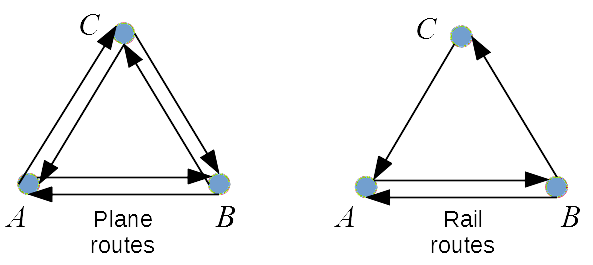
\includegraphics[width=2in]{relation-graphs.png}
\end{center}

Find the predicate expression that expresses this statement: 
"For the two given cities $x$ and $y$ there is a two-leg trip
using planes, but there is no two-leg trip using rail."\\
{\em Note.} We call a trip "two-leg", if it uses exactly two plane flights
or exactly two rail links. 
In this example all variables are from a 3-element set $\mathtt{City} = \{A,B,C\}$ 
\textendash{} see Figure. 


\noindent
{\bf (A)} $\forall x\;\forall y\; \forall z,\; \mathtt{Plane}(x,z) \wedge \mathtt{Plane}(z,y) \wedge$\\
$\neg \left( \mathtt{Rail}(x,z) \wedge \mathtt{Rail}(z,y) \right)$.\\[3pt]
{\bf (B)} $\exists z,\; \mathtt{Plane}(x,z) \wedge \mathtt{Plane}(z,y) \wedge$\\
$\neg \left(\mathtt{Rail}(x,z) \wedge \mathtt{Rail}(z,y)\right)$.\\[3pt]
{\bf (C)} $\forall x\; \forall y\; \exists z,\; \mathtt{Plane}(x,z) \wedge \mathtt{Plane}(z,x) \wedge$\\
$(\neg \mathtt{Rail}(x,z) \vee \neg \mathtt{Rail}(z,y))$.\\[3pt]
{\bf (D)} $\exists z_1\; \forall z_2,\; \mathtt{Plane}(x,z_1) \wedge \mathtt{Plane}(z_1,y) \wedge$\\
$(\neg \mathtt{Rail}(x,z_2) \vee \neg \mathtt{Rail}(z_2,y))$.





\subsection{Answers}

\vspace{6pt}
{\bf Question 1.} Answer {\bf (B),(C)}.\\
An obvious way to write DNF for this expression:
$$(X \wedge \neg Y \wedge Z) \vee (\neg X \wedge Y \wedge Z) \vee (\neg X \wedge \neg Y \wedge Z).$$
It contains one clause per every {\tt T} in the truth table. But it is not among the 
answers. Instead the answers {\bf (B)} and {\bf (C)} contain one shorter clause (with just two variables) that 
is equivalent to two clauses with three variables. For example, 
\begin{align}
 & (\neg Y \wedge Z) \equiv \nonumber \\
\equiv & \mathtt{True} \wedge (\neg Y \wedge Z) \equiv \nonumber \\
\equiv & (X \vee \neg X) \wedge (\neg Y \wedge Z) \equiv \nonumber \\
\equiv & (X \wedge (\neg Y \wedge Z)) \vee (\neg X \wedge (\neg Y \wedge Z)) \nonumber
\end{align}
Therefore the DNF can be written in a more compact form when we combine two blue clauses into
a shorter one:
$$\textcolor{blue}{(X \wedge \neg Y \wedge Z)} \vee (\neg X \wedge Y \wedge Z) \vee \textcolor{blue}{(\neg X \wedge \neg Y \wedge Z)} \equiv$$
$$\equiv \textcolor{blue}{(\neg Y \wedge Z)} \vee (\neg X \wedge Y \wedge Z)$$

\vspace{6pt}
{\bf Question 2.} Answer: {\bf (A)}, {\bf (D)}.\\
The variant {\bf (A)} lists all $3$ ways how $a \downarrow b$ can take value {\tt F}.\\
Variant {\bf (D)} $(\neg a) \wedge (a \vee \neg b)$ is the same thing. The clause $\textcolor{blue}{(\neg a)}$ 
there is equivalent to two clauses from {\bf (A)}: $\textcolor{blue}{(\neg a \vee \neg b) \wedge (\neg a \vee b)}$.

\vspace{6pt}
{\bf Question 3.} Answer: {\bf (B)}.\\
This means that there is a positive integer $M$ such that
for each $i \in \mathbb{Z}^{+}$ there would be $r \in \mathbb{Z}^{+}$ such that 
{\bf either} input $i$ is small ($i < M$) and program does not halt. 
{\bf Or} program $p$ outputs result $r$ upon receiving $i$ and 
that result is correct. (Note that even for small $i$ it is allowed
to stop and to output a correct answer: In this case $(i < M \,\wedge\, \neg H(p,i))$ is false, 
but $(A(p,i,r) \wedge C(i,r))$ is true.

Let us consider answer alternative {\bf (C)}:\\
$\forall p \in \mathcal{P}\; \exists M \in \mathbb{Z}^{+}\; \forall i \in \mathbb{Z}^{+}\;
\forall r \in \mathbb{Z}^{+},$\\
$((i > M \,\wedge\, H(p,i)) \vee (A(p,i,r) \wedge C(i,r)))$.

Note that for the answer {\bf (C)} (just like {\bf (A)} and {\bf (D)}) 
starts with $\forall p \in \mathcal{P}$. These statments contain 
$p$ as a {\em bound variable}; therefore they cannot express anything 
meaningful about the special $p$ mentioned in the English sentence: 
``For all inputs that are sufficiently large, {\bf the given program $p$}
halts and produces outputs.'' (The given Python program $p$ is not {\bf any program} or 
{\bf some program}; it is one certain program \textendash{} variable $p$ 
should have no quantifier.)

Even if we drop that $p \in \mathcal{P}$ the statement {\bf (C)} expresses 
something different: ``For a program there exists a number $M$ such that for all $i > M$ 
the program should halt. For any ``small'' input $i$ ($i \leq M$) it is not sufficient to halt; 
the program must be able to output {\bf any} result $r$ for the received input; 
and moreover \textendash{} that output should be correct:
$(A(p,i,r) \wedge C(i,r)))$.

\vspace{6pt}
{\bf Question 4.} Answer: {\bf (E)}.\\
Let us forget anything we know about Python programs and their halting. 
Let $H(p,i)$ be any predicate on elements of some set $p \in \mathcal{P}$ and  
positive integers $i$. We can prove that 
$(j > i \,\wedge\, (H(p,i) \rightarrow H(p,j))$ is always true. 
For the given $p$ take three different numbers $i_1,i_2,i_3$. Among 
$H(p,i_1)$, $H(p,i_2)$, $H(p,i_3)$ there are two values that are both true (or both false). 
Assign $i$ to the smallest of these $i_1,i_2,i_3$, and assign $j$ to the largest. 


\vspace{6pt}
{\bf Question 5.} Answer: {\tt 25,20,0,0}.\\
There are $5 \cdot 5 = 25$ ways to assign two students to five chairs
(you have to make a choice "1 of 5" two times).\\
Out of these $25$ functions there are $5$ functions that map both students
to the same chair ($c_1$, $c_2$, $c_3$, $c_4$, or $c_5$). All the other
$25-5 = 20$ functions that are injective (i.e. $f(s_1) \neq f(s_2)$).\\
Since there are more chairs than students, there are no surjective and bijective
functions.

\vspace{6pt}
{\bf Question 6.} Answer: {\bf (C)}.\\
The only option can be $x$ is the greatest common divisor of $y$ and $z$. 
$S(x,u,y)$ and $S(x,v,z)$ show that $x$ is {\bf some} common divisor of 
$y$ and $z$. And since $S(d,p,y) \wedge S(d,q,z) \rightarrow S(d,k,x)$ 
it means that another common divisor $d$ is also a divisor of $x$.\\
Therefore $x$ is the {\bf greatest} common divisor of $y$ and $z$. 

You can easily eliminate alternatives {\bf (B)}, {\bf (D)}, because
they state something about greatest common divisor of $p,q$ or $u,v$. 
But all these variables are {\bf bound} variables (they do not 
have any specific value; they vary over the whole set of positive integers). 


\vspace{6pt}
{\bf Question 7.} Answer: {\bf (D)}.\\
Note that the intermediate city $z_1$ for plane flights (that should exist)
has nothing common with the city $z_2$ for rail connections (that should not exist).
The conjunction {\bf BUT} means same as {\bf AND} from the logic point of view. 
We could express the answer like this:\\
$(\exists z_1,\; \mathtt{Plane}(x,z_1) \wedge \mathtt{Plane}(z_1,y))$ {\bf AND}\\
$\neg (\exists z_2,\; \mathtt{Rail}(x,z_2) \wedge \mathtt{Rail}(z_2,y))$. 

We can simpify the second clause using De Morgan's law:
$\forall z_2, (\neg \mathtt{Rail}(x,z_2) \vee \neg \mathtt{Rail}(z_2,y))$ and 
combine with the first clause by writing both quantifiers $\exists z_1$ and
$\forall z_2$ at the very front of the expression. 






\end{document}
